%% LyX 2.0.2 created this file.  For more info, see http://www.lyx.org/.
%% Do not edit unless you really know what you are doing.
\documentclass[letterpaper,twoside,english,compsoc]{IEEEtran}
\usepackage{helvet}
\usepackage[T1]{fontenc}
\usepackage[latin9]{inputenc}
\setlength{\parskip}{\smallskipamount}
\setlength{\parindent}{0pt}
\usepackage{graphicx}
\usepackage{setspace}
\setstretch{1.1000000000000001}

\makeatletter

%%%%%%%%%%%%%%%%%%%%%%%%%%%%%% LyX specific LaTeX commands.
\pdfpageheight\paperheight
\pdfpagewidth\paperwidth


%%%%%%%%%%%%%%%%%%%%%%%%%%%%%% Textclass specific LaTeX commands.
\newenvironment{lyxcode}
{\par\begin{list}{}{
\setlength{\rightmargin}{\leftmargin}
\setlength{\listparindent}{0pt}% needed for AMS classes
\raggedright
\setlength{\itemsep}{0pt}
\setlength{\parsep}{0pt}
\normalfont\ttfamily}%
 \item[]}
{\end{list}}

\@ifundefined{date}{}{\date{}}
%%%%%%%%%%%%%%%%%%%%%%%%%%%%%% User specified LaTeX commands.
\parindent 10pt

\markboth{IEEE TRANSACTIONS ON SOFTWARE ENGINEERING}{MCVEIGH ET AL.: INTRINSIC DEFINITION IN SOFTWARE ARCHITECTURE EVOLUTION}

\IEEEpubid{0000--0000/00\$00.00 \copyright 2007 IEEE}

\pagenumbering{gobble}

\makeatother

\usepackage{babel}
\begin{document}
\IEEEcompsoctitleabstractindextext{\small

\textbf{Abstract}---Incremental change is intrinsic to both the initial
development and subsequent evolution of large complex software systems.
We present an approach that captures this incremental change in the
definition of software architecture. The predominant advantage in
making the definition of evolution intrinsic to architecture description
is in permitting a principled and manageable way of dealing with unplanned
change and extension. We show how intrinsic definition also facilitates
decentralized evolution in which software is extended and evolved
by multiple independent developers. Further, we show how unplanned
extensions can be deployed to end users with the same facility that
plugins extensions are currently added to systems with planned extension
points. The approach is model-driven in that architecture definition
is used to directly construct both initial implementations and extensions
to these implementations. We have implemented intrinsic evolution
definition in Backbone - an architectural description language (ADL),
which has both a textual and a UML2, based graphical representation.
The paper uses Backbone to illustrate basic concepts through simple
examples and reports our experience in applying it and its associated
tool support to a larger example.\\
\begin{IEEEkeywords}

Software Architectures, Design Tools and Techniques

\end{IEEEkeywords}}\author{

Andrew McVeigh, Jeff Kramer and Jeff Magee

\IEEEcompsocitemizethanks{\IEEEcompsocthanksitem{

A. McVeigh, J. Kramer and J. Magee are with Imperial College London.

E-mail: \{a.mcveigh, j.kramer, j.magee\}@imperial.ac.uk

}}\thanks{

Manuscript received (insert date of submission if desired). Please
note that all acknowledgments should be places at the end of the paper,
before the bibliography.}}


\title{Intrinsic Definition in\\
Software Architecture Evolution}

\maketitle

\section{Introduction}

\IEEEPARstart{I}{NITIALLY} recognized by Boehm in his spiral model
of software development {[}{]} and more recently in agile development
methods {[}{]}, iterative and incremental software development is
fundamental to the delivery of complex software intensive systems.
As early as 1976, Belady and Lehman{[}{]} recognized that to retain
their usefulness, complex software systems are subject to continuous
incremental change throughout their lifetime. In 1991, Lehman{[}{]}
refined this observation and noted that systems are subject to incremental
growth due to the need to add functionality to maintain user satisfaction.
In summary, incremental change and extension can be regarded as intrinsic
to both the initial development and subsequent evolution of complex
software systems.

To deal with the increasing complexity of software systems, the Software
Engineering community has focused on dealing with systems at a level
of abstraction, known as software architecture {[}{]}. The software
architecture of a system deals with multiple views of a system including
both its functional and non-functional aspects. The central view is
the structural one in which a system is viewed as a set of components
that interact via connectors. Control of complexity is achieved by
hierarchical structure in which a component can be composed from subcomponents
with the leaf components of the hierarchy representing code modules.
A number of Architectural Description Languages (ADL) have been proposed
by the research community {[}{]}, and some of these have found their
way into commercial practice {[}{]}. While software architecture is
seen as an appropriate level for system redesign and restructuring
to permit change {[}{]}, the proposed ADLs do not deal directly with
evolution, considering it to be an extrinsic concern dealt with by
tools and processes external to those concerned with architecture
definition.

In this paper, we explore the alternative in which we regard evolution
as a concern that is intrinsic to architecture definition such that
the structural constructs we propose to capture change and extension
can be used during both initial development and subsequent evolution.
This intrinsic definition brings with it the requirement to deal with
unplanned extension, for it is impossible, whichever development process
is adopted, to foresee all possible future requirements for change
and evolution of a system.

Dealing with unplanned extension introduces a difficult dilemma in
designing constructs to support intrinsic definition. We would prefer
to have constructs that constrain change in such a way that their
application always results in structurally well formed and type correct
systems. However, such an approach inevitably means that only a subclass
of all possible valid change to a system is permitted. This is clearly
incompatible with dealing with unplanned extension since we cannot
predict the change that will be necessary. As a result, we have chosen
constructs that do permit changes that result in invalid systems;
however, we have ensured that these constructs are used in an environment
that comprehensively detects structural and type errors. In other
words, we combine the freedom to perform incorrect changes with the
ability to detect these errors so that we have sufficient expressiveness
to deal with unplanned changes. We permit change to be destructive
\textendash{} deleting elements of an architecture \textendash{} in
addition to being constructive \textendash{} adding elements to an
architecture.

In exploring intrinsic definition, we have considered the requirements
of distributed design and evolution in which development and extension
is carried out by different organizations. In particular, we are motivated
by the following situation which current approaches find problematic.
A development organization produces a software framework product that
is used by other organizations to build applications. In meeting their
local development requirements, these organizations may need to modify
and extend the framework to support their applications. The original
framework will evolve over time and the organizations that use it
need to apply their local changes to the framework before using the
evolved framework for their applications. In addition, a third party
may wish to use applications from more than one extenders of the framework
and thus need to merge changes from both these organizations and the
original framework provider. In the sequel, we examine the impact
of intrinsic definition on distributed evolution of this form.

If software architecture description is regarded only as design documentation,
a major problem arises in keeping this documentation in step with
the software implementation as a system evolves. We adopt a model
driven engineering approach in that architecture definition is not
just a documentation artifact but is a precise model used to directly
construct both initial implementations and extensions to these implementations.

In the following: Section 2 describes the key concepts for the intrinsic
definition of evolution in software architecture and explains their
use by mean of a simple example, Section 3 provides a more rigorous
definition of the these concepts and shows how they are computed over
a dependency graph of extensions, Section 4 recounts our experience
in using our prototype tool Evolve applied to a large case study and
evaluates the approach against the requirements for distributed evolution,
Section 5 discusses related work and finally Section 6 presents some
conclusions and directions for future work that build on the approach.


\section{Defining Change}

We first describe and motivate the key concepts we use to define change
in software architecture. Specifically, these constructs provide the
facility to remake a composition hierarchy. We demonstrate this in
a simple example described using our description language Backbone
in which the constructs have been implemented. It has both a graphical
form based on UML2 component diagrams and a textual form. The textual
form is simply a printed version of an XML representation used to
store and exchange Backbone definitions.


\subsection{Key Concepts}


\subsubsection*{\textmd{Resemblance}}

Resemblance defines a new component as the difference in structure
from one or more existing components. It is the delta, consisting
of the set of additions, deletions and replacements of the elements
of these components, that is applied to arrive at the new definition.
For a component, these elements are: parts \textendash{} instances
of subcomponents, ports \textendash{} instances of interfaces, connectors
\textendash{} bindings between ports, and attributes \textendash{}
component parameters. Resemblance may also be applied to interfaces
in which case the modified elements are operations. If a resemblance
delta consists only of additions then when applied to an interface,
it defines a proper subtype. The type inference and checking algorithm
we have implemented in our prototype tool Evolve takes full cognizance
of this.

Resemblance is a many to one relation to permit the merging of multiple
component definitions that may have arisen due to, for example, distributed
development. It might be of concern that if a sufficiently radical
delta is applied to a component then the new definition will bear
little or no resemblance, in the general sense, to the component definitions
from which it is derived. However, this is of more philosophical than
practical import as the primary intent of resemblance to record change
or evolution and we can find many examples in both engineering and
nature where things evolve dramatically from their original form.


\subsubsection*{\textmd{Replacement}}

Replacement globally substitutes the definition of one component for
another while preserving the identity of the original definition such
that any use relations that a larger system has with this definition
are preserved. When combined with resemblance, replacement permits
the incremental evolution of a component definition without necessarily
having to change the composite component definitions that use this
component.

Components and interfaces in the Backbone ADL are given globally unique
identifiers to permit the correct unambiguous application of replacement.
Replacement is the key to managing change in composite hierarchical
definitions since it permits substitution of component definitions
at one level of the composition hierarchy without necessarily affecting
higher layers.


\subsubsection*{\textmd{Stratum}}

A stratum is a package or module that holds the definitions relating
to an initial software architecture expressed as a composite component
or definitions relating to an evolution of that architecture. Each
stratum records the strata that it depends on such that to assemble
a system, the builder uses the current stratum and the transitive
closure of all strata that this stratum depends on. The computation
of resemblance in the context of the stratum dependency graph is addressed
in the next section.

In addition to extension, the stratum is the unit of sharing and ownership.
Each stratum is owned by a single party that has modification rights
to it. We can therefore use strata to model the ownership structure
of an architecture and map this onto a community of base and extension
developers. Our development tool Evolve and the Backbone runtime environment
support the import and export of strata for distributing extensions
and subsets of an architecture.

A stratum is also a unit of deployment in that its compiled version
together with associated component code can be sent to an end user
to extend their system in a similar fashion to Eclipse Plugins.\\


It should be noted that although resemblance allows elements to be
deleted in forming a new definition from existing defintions, this
is not destructive editing in the usual sense since the existing definition
is preserved and the deletion simply recorded in a delta. Our approach
preserves definitions and at no point overwrites old definitions with
new definitions. When replacing a definition from a base stratum with
a new definition using resemblance in an extension stratum, we do
not remove the base definition simply record the delta definition
in the extension stratum. Indeed, if we do not want a component definition
to be available for use in an extension, we simply replace it with
a resemblance delta that sets its retirement status to true.


\subsection{Example}

To illustrate the use of these three concepts we use the Singlelane
Bridge example from {[}{]}. This concurrent system models the access
of cars to a single lane bridge. Its component architecture can be
modeled in Backbone as shown in \ref{fig:SingleLaneBridge-components}.

\begin{figure}[h]
\noindent \begin{centering}
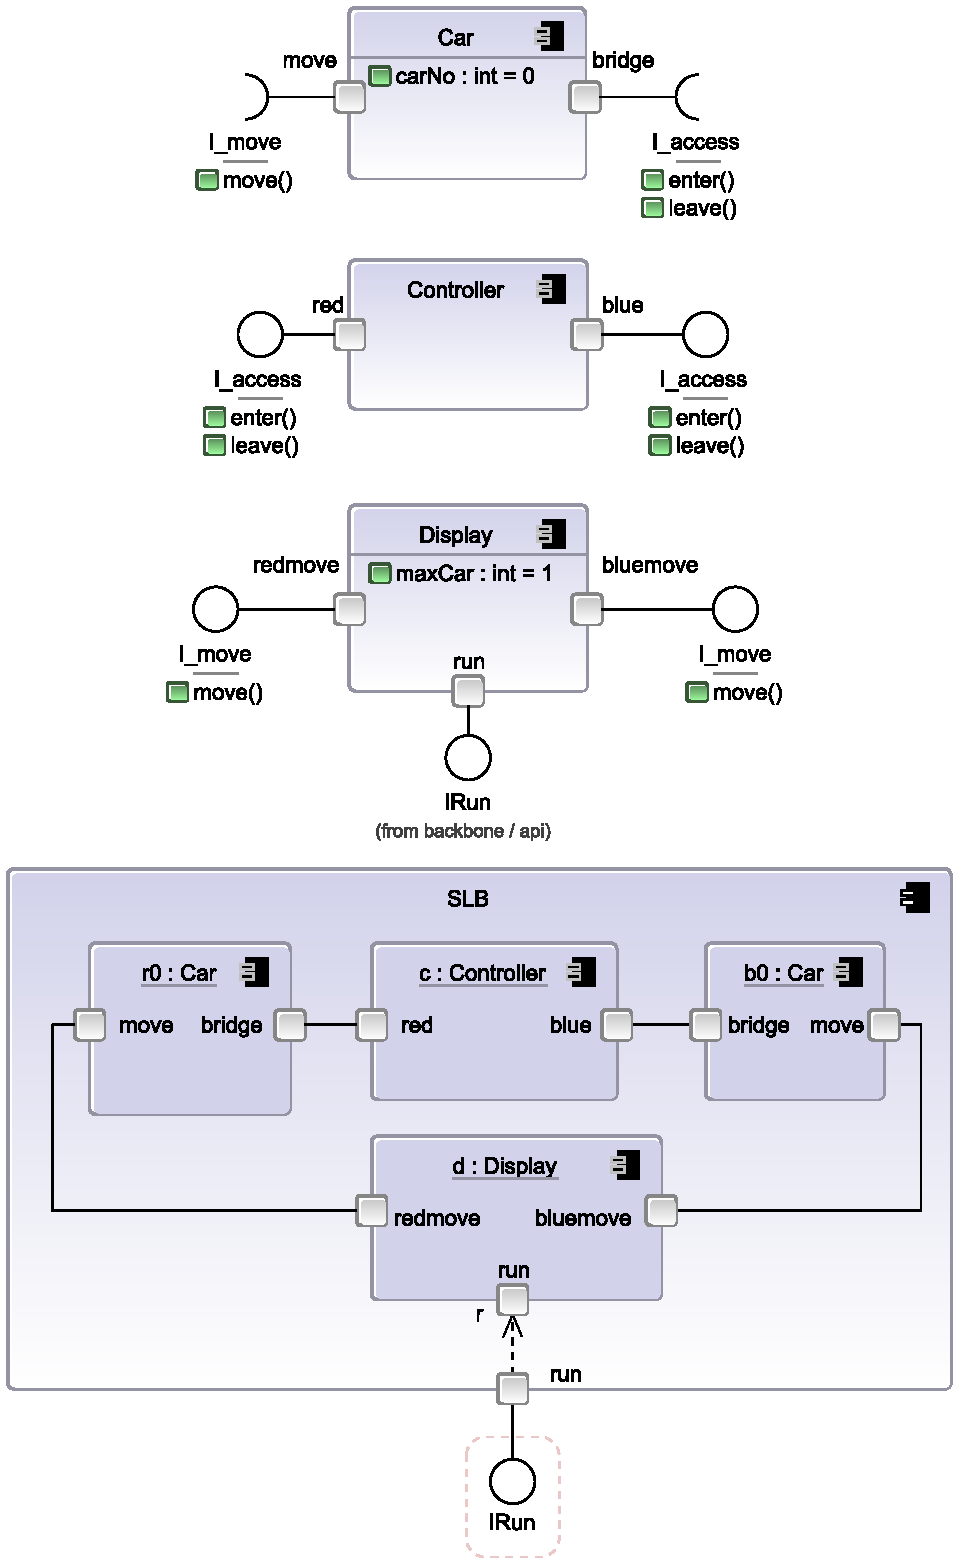
\includegraphics[width=1\columnwidth]{images/slb-components}
\par\end{centering}

\caption{\label{fig:SingleLaneBridge-components}SingleLaneBridge components}
\end{figure}


The textual architecture description that corresponds to this component
diagram is listed below:
\begin{lyxcode}
\textbf{\small stratum}{\small{}~Single\_Lane\_Bridge}{\small \par}

{\small{}~~}\textbf{\small depends-on}{\small{}~backbone}{\small \par}

{\small \{}{\small \par}

{\small{}~~~~}\textbf{\small interface}{\small{}~I\_access}{\small \par}

{\small{}~~~~~~}\textbf{\small implementation-class}{\small{}~bridge.I\_access}{\small \par}

{\small{}~~~~\{}{\small \par}

{\small{}~~~~~~}\textbf{\small operations:}{\small \par}

{\small{}~~~~~~~~enter;~leave;}{\small \par}

{\small{}~~~~\}}{\small \par}

{\small{}~~~~}\textbf{\small interface}{\small{}~I\_move}{\small \par}

{\small{}~~~~~~}\textbf{\small implementation-class}{\small{}~bridge.I\_move}{\small \par}

{\small{}~~~~\{}{\small \par}

{\small{}~~~~~~}\textbf{\small operations:}{\small \par}

{\small{}~~~~~~~~move;}{\small \par}

{\small{}~~~~\}}{\small \par}

{\small{}~~~~}\textbf{\small component}{\small{}~Controller}{\small \par}

{\small{}~~~~~~}\textbf{\small implementation-class}{\small{}~bridge.Controller}{\small \par}

{\small{}~~~~\{}{\small \par}

{\small{}~~~~~~}\textbf{\small ports:}{\small \par}

{\small{}~~~~~~~~red~}\textbf{\small provides}{\small{}~I\_access,}{\small \par}

{\small{}~~~~~~~~blue~}\textbf{\small provides}{\small{}~I\_access;}{\small \par}

{\small{}~~~~\}}{\small \par}

{\small{}~~~~}\textbf{\small component}{\small{}~Car}{\small \par}

{\small{}~~~~~~}\textbf{\small implementation-class}{\small{}~bridge.Car}{\small \par}

{\small{}~~~~\{}{\small \par}

{\small{}~~~~~~}\textbf{\small attributes:}{\small \par}

{\small{}~~~~~~~~carNo:~int~=~0;}{\small \par}

{\small{}~~~~~~}\textbf{\small ports:}{\small \par}

{\small{}~~~~~~~~move~}\textbf{\small requires}{\small{}~I\_move,}{\small \par}

{\small{}~~~~~~~~bridge~}\textbf{\small requires}{\small{}~I\_access;}{\small \par}

{\small{}~~~~\}}{\small \par}

{\small{}~~~~}\textbf{\small component}{\small{}~Display}{\small \par}

{\small{}~~~~~~}\textbf{\small implementation-class}{\small{}~bridge.Display}{\small \par}

{\small{}~~~~\{}{\small \par}

{\small{}~~~~~~}\textbf{\small attributes:}{\small \par}

{\small{}~~~~~~~~maxCar:~int~=~1;}{\small \par}

{\small{}~~~~~~}\textbf{\small ports:}{\small \par}

{\small{}~~~~~~~~redmove~}\textbf{\small provides}{\small{}~I\_move,}{\small \par}

{\small{}~~~~~~~~bluemove~}\textbf{\small provides}{\small{}~I\_move,}{\small \par}

{\small{}~~~~~~~~run~}\textbf{\small provides}{\small{}~IRun;}{\small \par}

{\small{}~~~~\}}{\small \par}

{\small{}~~~~}\textbf{\small component}{\small{}~SLB}{\small \par}

{\small{}~~~~\{}{\small \par}

{\small{}~~~~~~}\textbf{\small ports:}{\small \par}

{\small{}~~~~~~~~run~}\textbf{\small provides}{\small{}~IRun;}{\small \par}

{\small{}~~~~~~}\textbf{\small parts:}{\small \par}

{\small{}~~~~~~~~b0:~Car,}{\small \par}

{\small{}~~~~~~~~c:~Controller,}{\small \par}

{\small{}~~~~~~~~r0:~Car,}{\small \par}

{\small{}~~~~~~~~d:~Display;}{\small \par}

{\small{}~~~~~~}\textbf{\small connectors:}{\small \par}

{\small{}~~~~~~~~bb~}\textbf{\small joins}{\small{}~blue@c~}\textbf{\small to}{\small{}~bridge@b0,}{\small \par}

{\small{}~~~~~~~~br~}\textbf{\small joins}{\small{}~bridge@r0~}\textbf{\small to}{\small{}~red@c,}{\small \par}

{\small{}~~~~~~~~vr~}\textbf{\small joins}{\small{}~move@r0~}\textbf{\small to}{\small{}~redmove@d,}{\small \par}

{\small{}~~~~~~~~vb~}\textbf{\small joins}{\small{}~move@b0~}\textbf{\small to}{\small{}~bluemove@d,}{\small \par}

{\small{}~~~~~~~~r~}\textbf{\small delegates-from}{\small{}~run~}\textbf{\small to}{\small{}~run@d;}{\small \par}

{\small{}~~~~\}}{\small \par}

{\small \}}{\small \par}
\end{lyxcode}
This architecture represents a system with one red car and one blue
car, moving in opposite directions, competing for access to the bridge.
Access control is implemented by the Controller component, which provides
two I\_access interfaces. A Car calls enter to gain access to the
bridge and calls leave on exit. Cars display their movement using
the Display component. Note that all of the definitions are contained
in the SingleLaneBridge stratum that appears in Figure 3. Car, Controller
and Display are leaf components with an implementaion defined by Java
classes. SLB is a composite component that contains parts made from
these components interconnected by connectors to form the system.


\subsubsection*{\textmd{Using Resemblance}}

Now suppose that another developer wishes to evolve this system to
accommodate multiple red and blue cars moving in opposite directions.
This developer creates the stratum with the components shown in \ref{fig:MultiCarBridge-components}.
The developer defines three new components: CarFactory dynamically
creates a Car component when it receives an invocation on its creator
port, CarCreator is a leaf component that calls its create port maxCar
times, and finally, the composite component MultiCar creates nCars
Car components.

\begin{figure}[h]
\noindent \begin{centering}
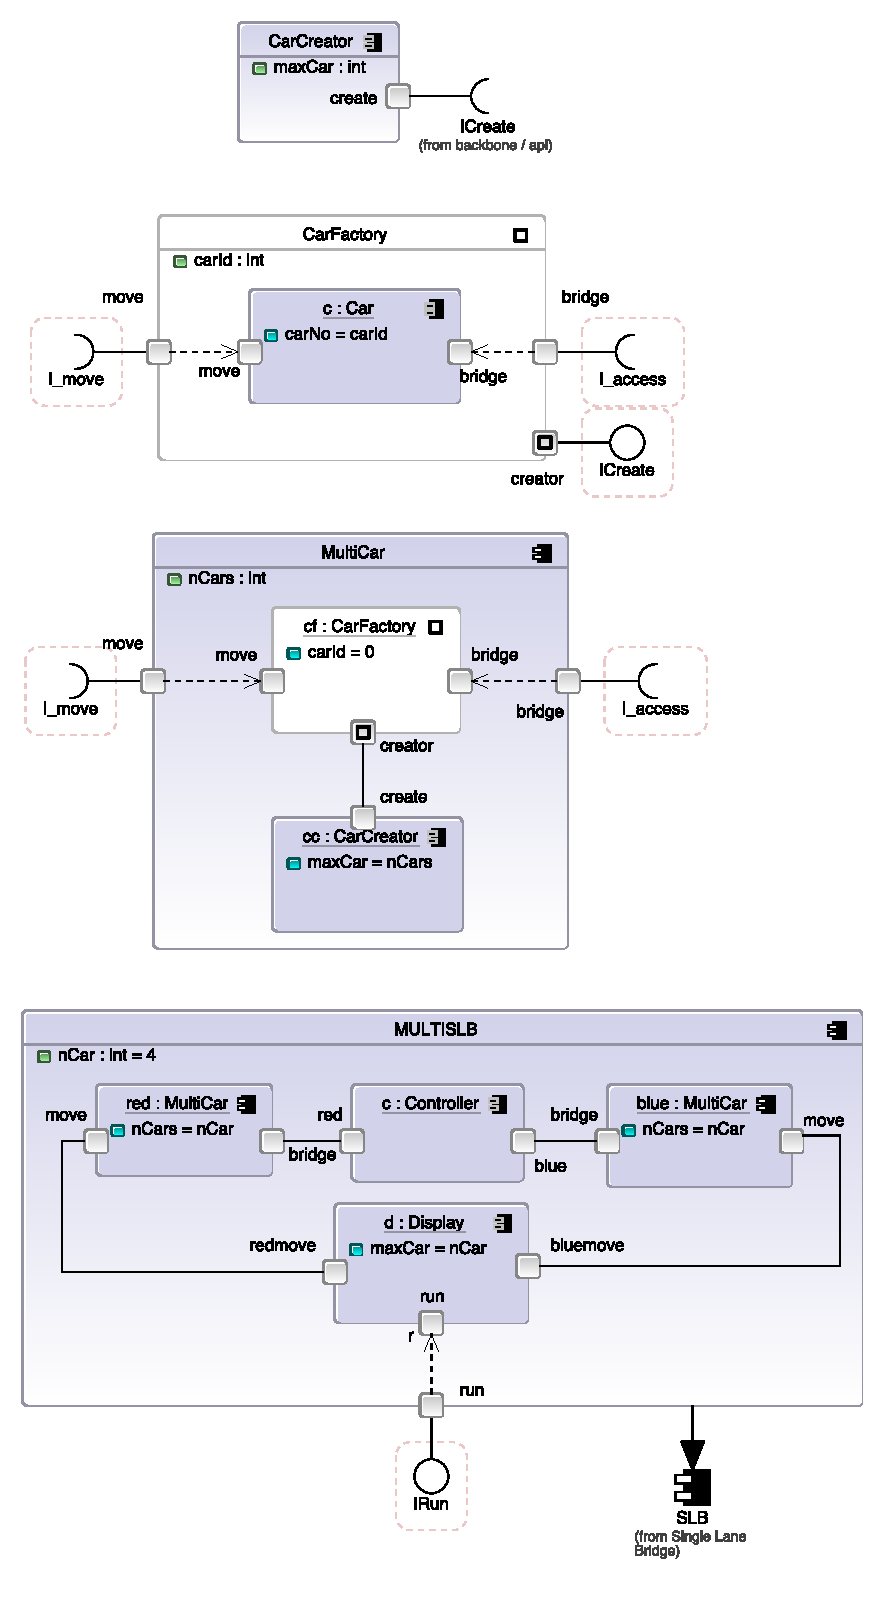
\includegraphics[width=1\columnwidth]{images/mlb-components}
\par\end{centering}

\caption{\label{fig:MultiCarBridge-components}MultiCarBridge components}


\end{figure}




The MULTSLB composite component is defined as a resemblance of the
SLB component from the SingleLaneBridge stratum. Graphically, resemblance
is depicted as a solid arrow pointing to an icon representing the
component from which the resemblance is derived. Although graphically
MULTSLB is depicted with all its component parts and connectors, in
fact as shown in the Backbone listing below, it is defined by a delta
that simply adds the nCar attribute and replaces the parts of type
Car with parts of type MultiCar. In addition, it replaces the instance
of Display with an instance of the same component type but with a
different attribute value. The new definition is formed graphically
by editing the previous definition that the Evolve tool displays when
the resemblance relation is established.
\begin{lyxcode}
\textbf{\small stratum}{\small{}~Multi\_Car\_Bridge}{\small \par}

{\small{}~~}\textbf{\small depends-on}{\small{}~Single\_Lane\_Bridge}{\small \par}

{\small \{}{\small \par}

{\small{}~~~~}\textbf{\small component}{\small{}~CarFactory~is-factory}{\small \par}

{\small{}~~~~~~~}\textbf{\small resembles}{\small{}~FactoryBase}{\small \par}

{\small{}~~~~\{}{\small \par}

{\small{}~~~~~~}\textbf{\small attributes:}{\small \par}

{\small{}~~~~~~~~~~carId:~int;}{\small \par}

{\small{}~~~~~~}\textbf{\small ports:}{\small \par}

{\small{}~~~~~~~~~~bridge,}{\small \par}

{\small{}~~~~~~~~~~move;}{\small \par}

{\small{}~~~~~~}\textbf{\small parts:}{\small \par}

{\small{}~~~~~~~~~~c:~Single\_Lane\_Bridge::Car}{\small \par}

{\small{}~~~~~~~~~~~~~~~}\textbf{\small slots:}{\small \par}

{\small{}~~~~~~~~~~~~~~~~~carNo~=~carId;}{\small \par}

{\small{}~~~~~~}\textbf{\small connectors:}{\small \par}

{\small{}~~~~~~~~~~b~}\textbf{\small delegates-from}{\small{}~move~}\textbf{\small to}{\small{}~move@c,}{\small \par}

{\small{}~~~~~~~~~~m~}\textbf{\small delegates-from}{\small{}~bridge~}\textbf{\small to}{\small{}~bridge@c;}{\small \par}

{\small{}~~~~\}}{\small \par}

{\small{}~~~~}\textbf{\small component}{\small{}~CarCreator}{\small \par}

{\small{}~~~~~~}\textbf{\small implementation-class}{\small{}~bridge.CarCreator}{\small \par}

{\small{}~~~~\{}{\small \par}

{\small{}~~~~~~}\textbf{\small attributes:}{\small \par}

{\small{}~~~~~~~~maxCar:~int;}{\small \par}

{\small{}~~~~~~}\textbf{\small ports:}{\small \par}

{\small{}~~~~~~~~create~requires~ICreate;}{\small \par}

{\small{}~~~~\}}{\small \par}

{\small{}~~~~}\textbf{\small component}{\small{}~MultiCar}{\small \par}

{\small{}~~~~\{}{\small \par}

{\small{}~~~~~~}\textbf{\small attributes:}{\small \par}

{\small{}~~~~~~~~nCars:~int;}{\small \par}

{\small{}~~~~~}\textbf{\small{}~ports:}{\small \par}

{\small{}~~~~~~~~bridge,}{\small \par}

{\small{}~~~~~~~~move;}{\small \par}

{\small{}~~~~~~}\textbf{\small parts:}{\small \par}

{\small{}~~~~~~~~cc:~CarCreator}{\small \par}

{\small{}~~~~~~~~~~}\textbf{\small slots:}{\small \par}

{\small{}~~~~~~~~~~~~maxCar~=~nCars,}{\small \par}

{\small{}~~~~~~~~cf:~CarFactory}{\small \par}

{\small{}~~~~~~~~~~}\textbf{\small slots:}{\small \par}

{\small{}~~~~~~~~~~~~carId~=~0;}{\small \par}

{\small{}~~~~~}\textbf{\small{}~connectors:}{\small \par}

{\small{}~~~~~~~~c~}\textbf{\small joins}{\small{}~create@cc~}\textbf{\small to}{\small{}~creator@cf,}{\small \par}

{\small{}~~~~~~~~b~}\textbf{\small delegates-from}{\small{}~bridge~}\textbf{\small to}{\small{}~bridge@cf,}{\small \par}

{\small{}~~~~~~~~m~}\textbf{\small delegates-from}{\small{}~move~}\textbf{\small to}{\small{}~move@cf;}{\small \par}

{\small{}~~~~\}}{\small \par}

{\small{}~~~~}\textbf{\small component}{\small{}~MULTISLB}{\small \par}

{\small{}~~~~~~}\textbf{\small resembles}{\small{}~Single\_Lane\_Bridge::SLB}{\small \par}

{\small{}~~~~\{}{\small \par}

{\small{}~~~~~~}\textbf{\small attributes:}{\small \par}

{\small{}~~~~~~~~nCar:~int~=~4;}{\small \par}

{\small{}~~~~~~}\textbf{\small replace-parts:}{\small \par}

{\small{}~~~~~~~~r0~}\textbf{\small becomes}{\small{}~red:~MultiCar}{\small \par}

{\small{}~~~~~~~~~~}\textbf{\small slots:}{\small \par}

{\small{}~~~~~~~~~~~~nCars~=~nCar}{\small \par}

{\small{}~~~~~~~~~~}\textbf{\small port-remaps:}{\small \par}

{\small{}~~~~~~~~~~~~move~}\textbf{\small maps-onto}{\small{}~xxx}{\small \par}

{\small{}~~~~~~~~~~~~bridge~}\textbf{\small maps-onto}{\small{}~xxx,}{\small \par}

{\small{}~~~~~~~~b0~}\textbf{\small becomes}{\small{}~blue:~MultiCar}{\small \par}

{\small{}~~~~~~~~~~}\textbf{\small slots:}{\small \par}

{\small{}~~~~~~~~~~~~nCars~=~nCar}{\small \par}

{\small{}~~~~~~~~~~}\textbf{\small port-remaps:}{\small \par}

{\small{}~~~~~~~~~~~~move~}\textbf{\small maps-onto}{\small{}~xxx}{\small \par}

{\small{}~~~~~~~~~~~~bridge~}\textbf{\small maps-onto}{\small{}~xxx,}{\small \par}

{\small{}~~~~~~~~d~}\textbf{\small becomes}{\small{}~d:~Single\_Lane\_Bridge::Display}{\small \par}

{\small{}~~~~~~~~~~}\textbf{\small slots:}{\small \par}

{\small{}~~~~~~~~~~~~maxCar~=~nCar;}{\small \par}

{\small{}~~~~\}}{\small \par}

{\small \}}{\small \par}
\end{lyxcode}
To produce this extension permitting multiple cars, some new program
source code must be written to implement the CarCreator component,
however, there is no requirement to access or modify any of the source
code relating to the base SingleLaneBridge stratum. Access to the
architecture description is sufficient to permit extension. Note that
resemblance is also used to define CarFactory, which extends FactoryBase
provided by the underlying backbone stratum. The stratum dependency
graph for the extension is shown in Figure \ref{fig:MultiCarBridge-strata-dependency}.

\begin{figure}[h]
\noindent \begin{centering}
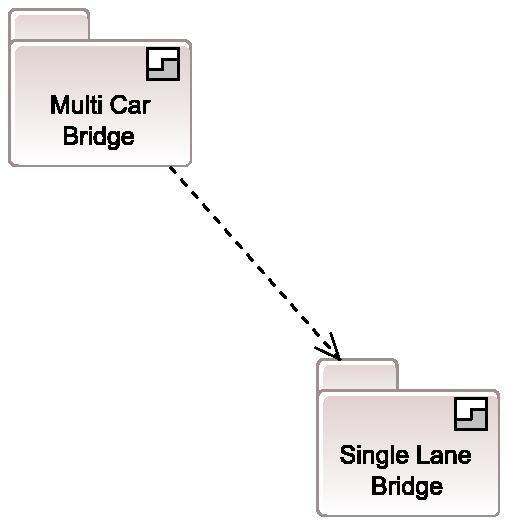
\includegraphics[width=0.5\columnwidth]{images/multicar-stratum}
\par\end{centering}

\caption{\label{fig:MultiCarBridge-strata-dependency}MultiCarBridge strata
dependency graph}


\end{figure}



\subsubsection*{Using Replacement}

The single lane bridge Controller component works well until the number
of cars increases to the point that a stream of cars, either red of
blue, continuously occupies the bridge denying access to cars moving
in the other direction. In other words, the Controller component is
safe but not fair. Figure \ref{fig:FairBridge-replacement-controlle}
shows how a revised Controller that does implement fairness is introduced.

\begin{figure}[h]
\noindent \begin{centering}
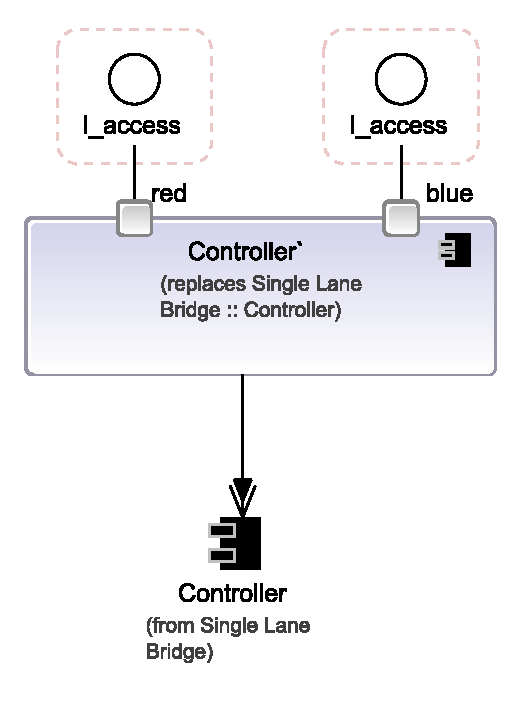
\includegraphics[width=0.5\columnwidth]{images/fair-controller}
\par\end{centering}

\caption{\label{fig:FairBridge-replacement-controlle}FairBridge replacement
controller}
\end{figure}


The listing below shows the Backbone textual represenation of the
evolved controller.
\begin{lyxcode}
{\small }%
\begin{minipage}[t]{1\columnwidth}%
\begin{lyxcode}
\textbf{\small stratum}{\small{}~Fair\_Bridge}{\small \par}

{\small{}~}\textbf{\small depends-on}{\small{}~Single\_Lane\_Bridge}{\small \par}

{\small \{}{\small \par}

{\small{}~}\textbf{\small component~}{\small Controller}{\small \par}

{\small{}~~}\textbf{\small implementation-class}{\small \par}

{\small{}~~~~bridge.FairController}{\small \par}

{\small{}~~}\textbf{\small resembles~}{\small Single\_Lane\_Bridge::Controller}{\small \par}

{\small{}~}\textbf{\small{}~replaces~}{\small Single\_Lane\_Bridge::Controller}{\small \par}

{\small{}~~\{}{\small \par}

{\small{}~~\}}{\small \par}

{\small \}}\end{lyxcode}
%
\end{minipage}{\small \par}
\end{lyxcode}
Replacement is so often combined with resemblance that we use a single
graphical symbol (combined solid and fishbone arrow) to indicate this
combination as shown in figure \ref{fig:FairBridge-replacement-controlle}.
The diagram and text show that we are replacing Controller with a
component that resembles it exactly with the exception of the implementation
class that we have changed. We can now combine this fair bridge controller
with the MultiCarBridge stratum as shown in Figure 5. The stratum
FairMultiCarBridge represents a system that permits multiple cars
and has a fair controller. The stratum contains no definitions of
components or deltas; it simply indicates its dependences as shown
in the Backbone text below Figure \ref{fig:FairMultiLaneBridge-strata-depen}.

\begin{figure}[h]
\noindent \begin{centering}
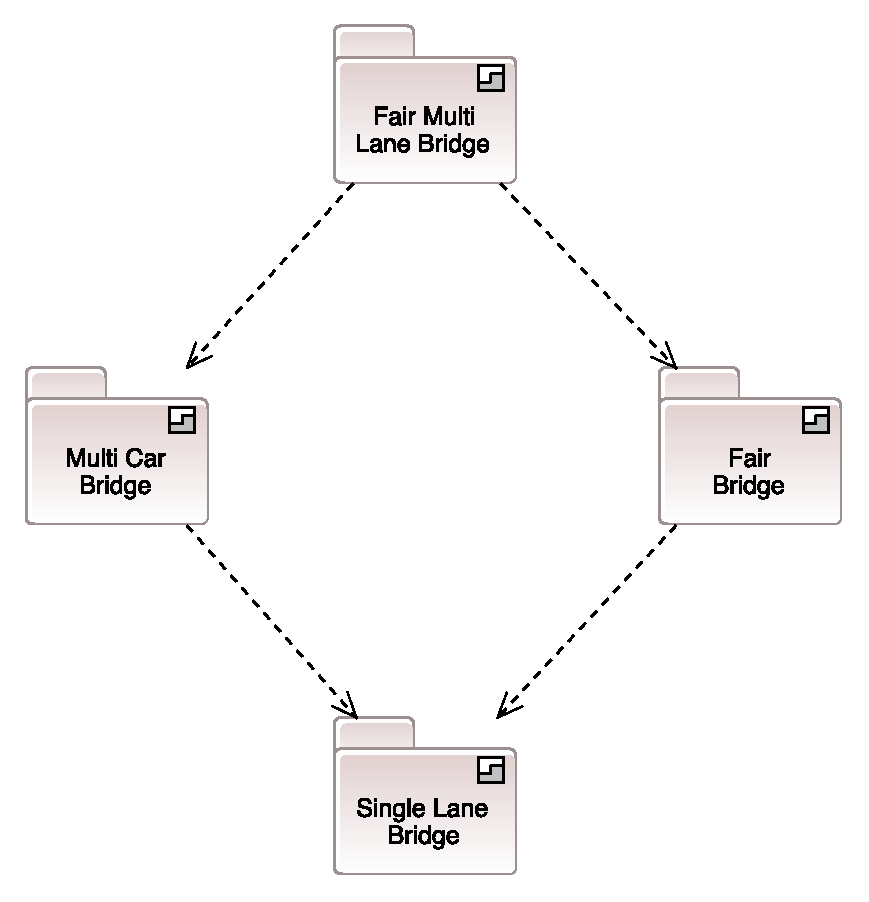
\includegraphics[width=0.87\columnwidth]{images/all-strata}
\par\end{centering}

\caption{\label{fig:FairMultiLaneBridge-strata-depen}FairMultiLaneBridge strata
dependency graph}
\end{figure}

\begin{lyxcode}
\textbf{\small stratum}{\small{}~Fair\_Multi\_Lane\_Bridge}{\small \par}

{\small{}~~}\textbf{\small depends-on~}{\small Multi\_Car\_Bridge,~Fair\_Bridge}{\small \par}

{\small \{}{\small \par}

{\small \}}{\small \par}


\end{lyxcode}
Figure \ref{fig:FairMultiLaneBridge-strata-depen} illustrates how
strata are merged. This can of course lead to conflicts in definitions,
which we discuss in the next section. In the case of the example,
a more plausible scenario would be for the original base developer,
or a third party, to export this new stratum to the multi-car developer
who could import it as shown in Figure \ref{fig:Alternative-dependency-graph}.
If we were to write out the Backbone text again, it would now show
a dependency on FairBridge rather than SingleLaneBridge for MultiCarBridge.
\begin{figure}[h]
\noindent \begin{centering}
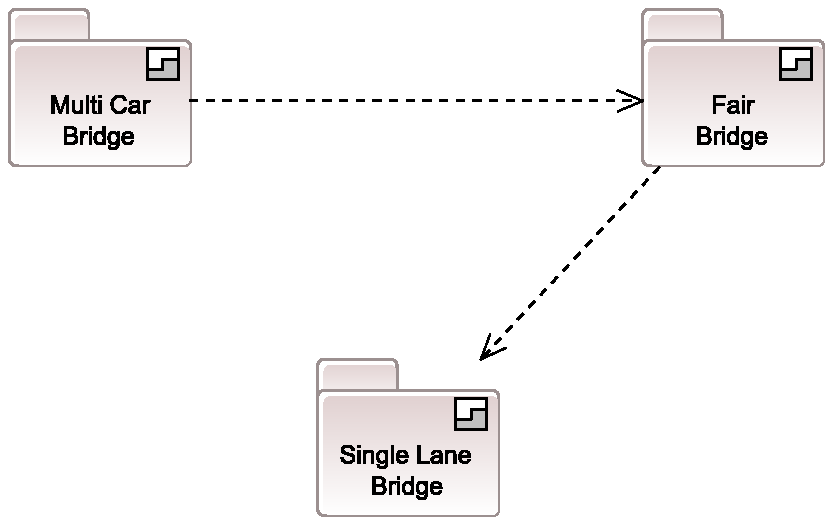
\includegraphics[width=0.8\columnwidth]{images/alternative-graph}
\par\end{centering}

\caption{\label{fig:Alternative-dependency-graph}Alternative dependency graph}


\end{figure}



\section{Intrinsic Definition in Practice}

Proposers of a new approach to software architecture description have
the responsibility to demonstrate that it can be put into industrial
practice. In this section, we discuss three significant barriers to
doing so and outline how they are addressed. They are: tool support,
compatibility with existing libraries and toolkits, and application
to existing legacy software.


\subsection{Tool Support}

The Backbone ADL is supported by a graphical modeling tool Evolve
and a runtime environment which instantiates and interconnects components
from a Backbone description. Figure 7 is an overview of the elements
that make up the modeling tool and runtime environment. The DeltaEngine
layer implements the resemblance algorithm described in the previous
section and is used in the modeling tool to build graphical representations
of composite components from delta definitions and in the runtime
environment to instantiate components from these same delta definitions.
In addition to this interpreted runtime the modeling tool can optionally
compile a \textquotedblleft{}flat\textquotedblright{} description
of the model as a builder class. In this case, no runtime environment
is required. It should be noted that even the interpreted runtime
environment incurs no overhead during execution of a system; it is
only active at startup time when it directs instantiation and interconnection.
\end{document}
